
{\underline {\bf В третьей главе}} описана разработанная
модель РС, основанная на применении теории нечетких множеств
(далее будем обозначать разработанную модель НРС) и проведено теоретическое
сравнение этой модели с АКМ.\\

Будем представлять контент как нечеткое подмножество множества характеристик и
определим операции объединения и пересечения контентов:
\begin{itemize}
			\item
				$c_X(u) = \{(x | w_U(u, x )) \}, w_U(u, x) \in [0,1]$ ---
				контент пользователя, $x \in X$. При этом множество $X$ не
				обязательно является множеством $I$, как в случае с АКМ, а,
				например, в качестве характеристик может выступать контекстная
				информация.
				$w_U(u, x)$ является
				характеристической функции принадлежности;
			\item
				$c_Y(i) = \{(y | w_I(i, y )) \}, w_I(i, y) \in [0,1]$ ---
				контент объекта, $y \in Y$.
				$w_I(i, x)$ является
				характеристической функции принадлежности;
			\item
				$c_X(u) = \varnothing$, если $w_U(u, x) \equiv 0$ ---
				пустой контент пользователя;
			\item
				$c_Y(i) = \varnothing$, если $w_I(i, y) \equiv 0$ ---
				пустой контент объекта;
			\item
				$c_X(u_1) \bigcup c_X(u_2) = c_X(v): \forall x \in X$ $w_U(v, x) =
				\max(w_U(u_1, x), w_U(u_2, x))$ ---
				объединение контентов пользователей;
			\item
				$c_Y(i_1) \bigcup c_Y(i_2) = c_Y(j): \forall y \in Y$ $w_I(j, y) =
				\max(w_I(i_1, y), w_I(i_2, y))$ ---
				объединение контентов объектов;

			\item
				$c_X(u_1) \bigcap c_X(u_2) = c_X(v): \forall x \in X$ $w_U(v, x) =
				\min(w_U(u_1, x), w_U(u_2, x))$ ---
				пересечение контентов пользователей;
			\item
				$c_Y(i_1) \bigcap c_Y(i_2) = c_Y(j): \forall y \in Y$ $w_I(j, y) =
				\min(w_I(i_1, y), w_I(i_2, y))$ ---
				пересечение контентов объектов.
\end{itemize}

В качестве меры близости объектов будем использовать обобщенное расстояние Хэмминга:
    \begin{equation}
		\label{fuz:rhu}
		\rhu(u,v) =
      \begin{cases}
		  \text{Не определено, если} & c_X(u) \bigcap c_X(v) = \varnothing\\
		  \frac{1}{|X|} \cdot \sum \limits_{x \in X} |w_U(u, x) -
		  w_U(v,x)| & \text{иначе}
      \end{cases}
    \end{equation}

В качестве меры близости пользователей будем использовать обобщенное расстояние Хэмминга:
    \begin{equation}
		\label{fuz:rhi}
		\rhi(i, j) =
      \begin{cases}
         \text{Не определено, если} & c_Y(i) \bigcap
		  c_Y(j) = \varnothing \\
        \frac{1}{|Y|} \cdot \sum \limits_{y \in Y} |w_I(i, y) - w_I(j,y)| & \text{иначе}
      \end{cases}
    \end{equation}
Заданные расстояния обладают метрическими свойствами.

Определим отношение близости пользователей:
\begin{equation}
	\label{fuz:ru}
	u \ru v \Leftrightarrow \rhu(u, v) \le \varepsilon^{\prime}_p :=
	\varepsilon_p.
\end{equation}

Определим отношение близости объектов:
\begin{equation}
	\label{fuz:rt}
i \rt j \Leftrightarrow \rhi(i, j) = \varepsilon_0 := 0.
\end{equation}

Современные РС могут оперировать с контекстной информацией,
а не только информацией о предпочтениях пользователя как
в случае с АКМ.
Этой информацией может быть, к примеру,
социально-демографические данные пользователя или данные о
географическом местоположении.
Разработанная модель позволяет работать
с подобной информацией, поэтому разработанная модель является расширением
АКМ по данным о пользователе. РС производит сопоставление
информации о пользователе и объекте, за счет которого определяется
оценка близости пользователя и объекта. В случае АКМ сопоставление
определяется эвристическими утверждениями.
При работе с более широкой и
неоднозначной информацией о пользователе и при ее сопоставлении с данными об
объектах могут применяться знания эксперта, алгоритмические подходы такие, к примеру,
как машинное обучение и т.д.

В разработанной модели сопоставление информации и пользователе и объекте
определяется заданием
нечеткого отображения $\dc: X \times Y \rightarrow [0,1]$, именуемым оценкой
близости характеристик.

Функция сходства $\dc$ может быть задана в табличной или
аналитической форме алгоритмически или экспертом.

Зададим функцию принадлежности при нечетком отображении $\Psi$ следующим образом:
\begin{equation}
	\label{make-rho1}
		\nu_{\Psi}(y) = \underset{x \in X} {\mathrm{\max}} \min\{
			\delta_c(x,y); w_U(u, x) \}
\end{equation}

С помощью функции $\dc$ можно определить нечеткое отображение $\Psi: X \rightarrow Y$ контента
пользователя на множество контентов объектов.
Для этого
зададим характеристическую функцию принадлежности $\nu_{\Psi}$ характеристики
$y$ нечеткому подмножеству универсального множества $Y$ при отображении $\Psi$ следующей формулой:
\begin{equation}
	\nu_{\Psi}(y) = \underset{x \in X} {\mathrm{\max}} \min\{ \rho(x,y); \mu(x) \}
\end{equation}

Определим функцию отображения контентов пользователей:
\begin{equation}
	\Psi(c_X(u)) = \{ (y | \nu_{\Psi}(y)) \}, y \in Y
\end{equation}

При наличии способа отображения контента пользователя, зададим расстояние
между пользователем $u$ и объектом $i$, значение которого будет выступать в
роли значения прогнозной функции:
	\begin{equation}
		\label{my-rh}
		\rh(u,i) := \rhi(\overline{i}, i)\text{, где }
		c_Y(\overline{i}) := \Psi(c_X(u))
	\end{equation}

\begin{equation}
	\begin{aligned}
	\label{my-pi}
		\text{Нечеткое правило $\Pi_f$ НРС }\\
	\text{заключается в задании оценки сходства } \delta_c\\
	\text{и в дальнейшем расчете прогнозной функции }\rh
	\end{aligned}
\end{equation}

%Будем говорить, что правило вывода $\Pi_f$ задано аккуратно, если
%выполняется следующее неравенство:
%\begin{equation}
%	\label{acc}
%	|\rho(u, i) - \rh(u, i)| \le \varepsilon_p
%\end{equation}



%% Пусть мы обладаем алгоритмом, вычисляющим расстояние $\rho_{1}(a, i)$ по некоторым характеристикам пользователя и объекта так, что:
%% \begin{equation}\label{rho-pro}
%% |\rho_{1}(a, i) - \rho_0(a, i)| \le \varepsilon_0 \in \varepsilon(0)
%% \end{equation}
%% где $\rho$ является {\it метрической} функцией расстояния. 
%% %При расчете расстояния характеристиками пользователя могут выступать не только его оценки, как для существующих эвристических РС. 
%% %К примеру, пользователь перед работой с РС может заполнить анкету\cite{bank}, которая состоит из характеристик, присущих также и 
%% %объектам, или из характеристик, которые сопоставимы с характеристиками объектов. 
%% %К примеру, это может набор кинематографических жанров, которые интересны пользователю и 
%% %характерны для фильмов. 
%% Способ задания такой функции $\rho$ для РС, а также
%% плюсы использования таких функций выходит за рамки текущей статьи, однако данные вопросы были раскрыты. 
%Процесс решения задач РС можно рассматривать как формирование
%прототипа контента $\overline{u}_a$ активного пользователя $u$
%при представлении
%контента пользователя в виде нечеткого
%подмножества множества объектов:
%$c_X(u_a) = \{ (i | \rho(u_a, i))\}$, $\rh(u_a, i) \not \in P_0$
%$\rho(u_a, i)$ --- выступает в роли характеристической функции.
%$I$ --- множество характеристик.
%
%Прототип контента:
%$c_X(\overline{u}_a) = \{ (i | \rh(\overline{u}_a, i))\}$, $\rho(\overline{u}_a, i) \not \in P_0$
%$\rh(\overline{u}_a, i)$ --- выступает в роли характеристической функции.
%$I$ --- множество характеристик.
%
%Тогда качество решения можно рассматривать как расстояние между реальным
%контентом и его прототипом.
%	%21
%Введем оценку решения любой из задач как обобщенное
%расстояние Хэмминга между прототипом и реальным контентом:
%		\begin{equation}
%			\label{my-e}
%		\mathcal{E} =
%			\frac{1}{|\overline{P}_{\bot}|} \cdot \sum \limits_{u_a} \sum
%			\limits_{k=1}^{|c_X(\overline{u}_a)|} |\rh(\overline{u}_a, i_k) -
%			\rho(u_a, j_k)|
%			\end{equation}
%		\begin{itemize}
%			\item $i_k = j_k = i_{\bot}$ для задачи прогнозирования.
%			\item $c_X(u_a), c_X(\overline{u}_a)$ упорядочены по возрастанию
%				$\rho(u_i, j_k)$, $\rh(\overline{u}_a, i_k)$ соответственно для
%				оценки задачи $topN$.
%		\end{itemize}
%
%Оценка обладает метрическими свойствами и поэтому может быть
%применена как количественный показатель.
%Введенная оценка, как показано в диссертационном исследовании,
%коррелирует с использующимися оценками решения задач $topN$ и прогнозирования.
%Ее применение
%не ограничено свойствами исходных данных, что характерно для
%использующихся оценок решения задачи $topN$, и она может применяться для
%любой задачи. Поэтому данная оценка названа обобщенной и может служить
%стандартом оценки решения при условии аккуратного определения $\delta_c$.
Определим НРС следующим образом:
	\begin{multline}
		(c_X(u) = \{(x | w_U(u, x )) \},\\
		 c_Y(i) = \{(y | w_I(i, y )) \},\\
		\Pi \in \{\Pi_{O}, \Pi_{C}, \Pi_f\}
	\end{multline}
НРС включает правила вывода АКМ,
и поэтому является ее расширением.

{\bf Решения задач в нечеткой модели}.
Определим решения в НРС при использовании $\Pi_f$. Задача $topN$ может быть решена
с помощью линейного поиска объектов, близких к активному пользователю.
Задача прогнозирования заключается в вычислении расстояния $\rh(u_a, i_{\bot})$ между
активным пользователем и прогнозируемым объектом.
%Условием, при котором
%нечеткая модель гарантирует получение качественного решении при использовании $\Pi_f$
%является аккуратность задания $\Pi_f$ (\ref{acc}).

При решении задачи $topN$ максимальное число вычислений $\rh$ равно $n$,
поэтому асимптотическая сложность алгоритма решения равна $O(n)$. Для решения
задачи $pred$ единожды проводится вычисление расстояния,
поэтому асимптотическая сложность алгоритма решения равна $O(1)$.

Проведем сравнение эффективности НРС и АКМ.

{\bf Сравнение моделей по критерию вычислительной сложности}.
В таблице <<Сравнение асимптотических сложностей>> (\ref{tbl:complex})
приведены асимптотически сложности алгоритмов решений задач в АКМ и НРС.

\begin{table}[h]
	\caption{Сравнение асимптотических сложностей}
	\label{tbl:complex}
  \begin{center}
  \begin{tabular}{|c|c|c|c|}
	\hline
	Модель & Задача & Сложность  \\ \hline
	АКМ & $topN$ & $O(n^2)$  \\ \hline
	АКМ & Прогнозирование & $O(m)$ \\ \hline
	НРС & $topN$ & $O(n)$ \\ \hline
	НРС & Прогнозирование & $O(1)$ \\ \hline
  \end{tabular}
\end{center}
\end{table}
Асимптотические сложности решений задач в НРС
при использовании правила $\Pi_f$ на порядок меньше сложностей
КМ, поэтому разработанная модель эффективнее по критерию
вычислительной сложности.

{\bf Сравнение моделей по критерию качества решения}.
Рассмотрим эффективность решений задач по критерию качества
в НРС при использовании $\Pi_O$ и $\Pi_C$.

При решении задачи $pred$ в НРС при применении $\Pi_C$
будем строить кластер соседей следующим образом:
$\mathcal{N}_U = \{ u : \rhu(u_a, u) \le \frac{1}{2} \cdot \varepsilon_p \wedge
(u, i_{\bot}, \rho(u, i_{\bot})) \in P_0)$ \}.
При таком построении кластера выполняется
достаточное условие эффективности решения,
что обусловлено
метрическими свойствами используемой в НРС
меры близости $\rhu$ (\ref{fuz:rhu}).
%Покажем, что выполняется достаточное условие. Напомним, что оно
%заключается в выполнении свойства транзитивности отношения близости $\ru$ на
%кластере соседей.
%$\forall u, v \in \mathcal{N}_U$ верно, что
%$(u_a \ru u) \wedge (u_a \ru v)$. Так как функция $\rhu$ обладает
%метрическими свойствами, то $\rhu(u, v) \le \rhu(u_a, u) + \rhu(u_a, v)$.
%По дополнительному условия
%$\rhu(u_a, u) \le \frac{1}{2} \cdot \varepsilon_0$,
%$\rhu(u_a, v) \le \frac{1}{2} \cdot \varepsilon_0$,
%поэтому $\rhu(u, v) \le \varepsilon_p \Rightarrow u \ru v$.

При решении задачи $topN$ в НРС при применении $\Pi_O$
выполняется достаточное условие эффективности решения,
что обусловлено заданием отношения $\rt$ (\ref{fuz:rt})
в НРС и метрическими свойствами используемой в
НРС меры близости $\rhi$ (\ref{fuz:rhi}).

Так как в НРС при использовании $\Pi_C$ и $\Pi_O$
выполняются достаточные условия эффективности решений, то
разработанная модель является эффективной модификацией АКМ.

Эффективность НРС по критерию качества при применении правила
вывода $\Pi_f$ так же, как и в АКМ ограничена
дополнительным условием.
В обеих моделях выполнение условий
зависит от разработчика: для АКМ это выбор функции $\rhi, \rhu$ и порогового
значения $\varepsilon_i, \varepsilon_u$, для НРС --- это
определение $\delta_c$.
Однако при работе с АКМ
разработчик обладает меньшей свободой действий, чем при работе с
НРС, так как он может варьировать только функцию, которая будет
использоваться в качестве меры близости, и ее пороговое значение.
При работе с НРС разработчик может варьировать
алгоритмы, эвристики, наборы данных, знания
экспертов и т.п., чтобы задать $\delta_c$ и зависящее от этой функции $\Pi_f$.

{\bf Сравнение моделей по критерию стабильности}.
Эффективность по качеству решений, получаемых в АКМ зависит от свойств исходных
данных, поэтому АКМ неэффективны по критерию стабильности. В том числе, если
мощность $P$ мала или вовсе равна нулю, то АКМ нельзя применять для
решения.

При применении
правила вывода $\Pi_f$ в НРС эффективность по качеству решения
не зависит от свойств исходных данных, зависит только от разработчика.

%Напомним, что оно
%заключается в выполнении свойства транзитивности отношения близости $\rt$ на
%множестве $I^a_0 \bigcup I_{\bot} \bigcup I_{topN}$.
%Покажем, что $(i_0 \rt i) \wedge (i_0 \rt i_{\bot}) \Rightarrow i_{\bot} \rt
%i$. Отношение $i_0 \rt i_{\bot}$ выполняется по эвристическому утверждению ООМ
%(\ref{ors-assert}), отношение $i_0 \rt i$ выполняется по построению решения.
%Так как функция $\rhi$ обладает метрическими
%свойствами, то $\rhi(i, i_{\bot}) \le \rhi(i_0, i) + \rhi(i_{\bot}, i_0)$.
%По дополнительному условию $\rhi(i_0, i) = 0$,
%так как выполняется  $i_0 \rt i_{\bot}$, то $\rhi(i_0, i_{\bot}) \le
%\varepsilon_0$. Поэтому $\rhi(i, i_{\bot}) \le \varepsilon_0$, то есть
%выполняется отношение $i \rt i_{\bot}$.

%$\mathcal{E}^1_{task} < \mathcal{E}^2_{task}$, где
%$\mathcal{E}^1_{task}$ --- значение оценки, полученное на решении задач при
%использовании нечеткой коллаборативной модели,
%$\mathcal{E}^2_{task}$ --- значение оценки, полученное на решении задач при
%использовании коллаборативной модели.

%%%%%%%%%%%%%%%%%%%%%%%%%%%%% MOD
%В диссертационном исследовании была введена модификация алгоритма составления
%кластера соседей при решении задачи прогнозирования с использованием $\Pi_C$. Данная модификация
%гарантирует выполнение достаточного условия для любых значений $\varepsilon_p$,
%не обязательно близких нулю, за счет чего при реализации РС становится
%возможным достичь выполнения достаточного условия при различных требованиях к
%РС. Опишем модификацию.
%
%Зададим пользователя, который является объединением всех пользователей,
%принадлежащих кластеру:
%$u_{\bigcup} = (\bigcup \limits_{u \in \mathcal{N}_U} u) \bigcup u_a$.
%
%Зададим пользователя, который является пересечением всех пользователей,
%принадлежащих кластеру:
%$u_{\bigcap} = (\bigcap \limits_{u \in \mathcal{N}_U} u) \bigcap u_a$.
%
%Модификация алгоритма заключается в том, что добавляется дополнительное условие на
%занесение соседа $u$ в кластер (алгоритм представлен на Рис.
%\ref{pis:method},
%где $M$ в блок-схеме является максимальным числом соседей):
%\begin{equation*}\label{method}
%	u \ru u_a \wedge u \ru u_{\bigcup} \wedge u \ru u_{\bigcap}
%\end{equation*}
%
%Данный алгоритм является более эффективным по критерию качества решения,
%чем алгоритм решения задачи прогнозирования АКМ, так как выполняется
%достаточное условие.
%Теоретически $\mathcal{E}^1_{p} < \mathcal{E}^2_{p}$, где
%$\mathcal{E}^1_{p}$ --- значение оценки, полученное на решении задачи
%прогнозирования при
%использовании модифицированного алгоритма составления кластера соседей,
%$\mathcal{E}^2_{p}$ --- значение оценки, полученное на решении задачи
%прогнозирования при
%использовании стандартного алгоритма составления кластера соседей.

%\begin{figure}[H]
%	\begin{center}
%		\label{pis:method}
%	\caption{Модификация построения кластера соседей при решении задачи
%	прогнозирования в нечеткой коллаборативной модели}
%  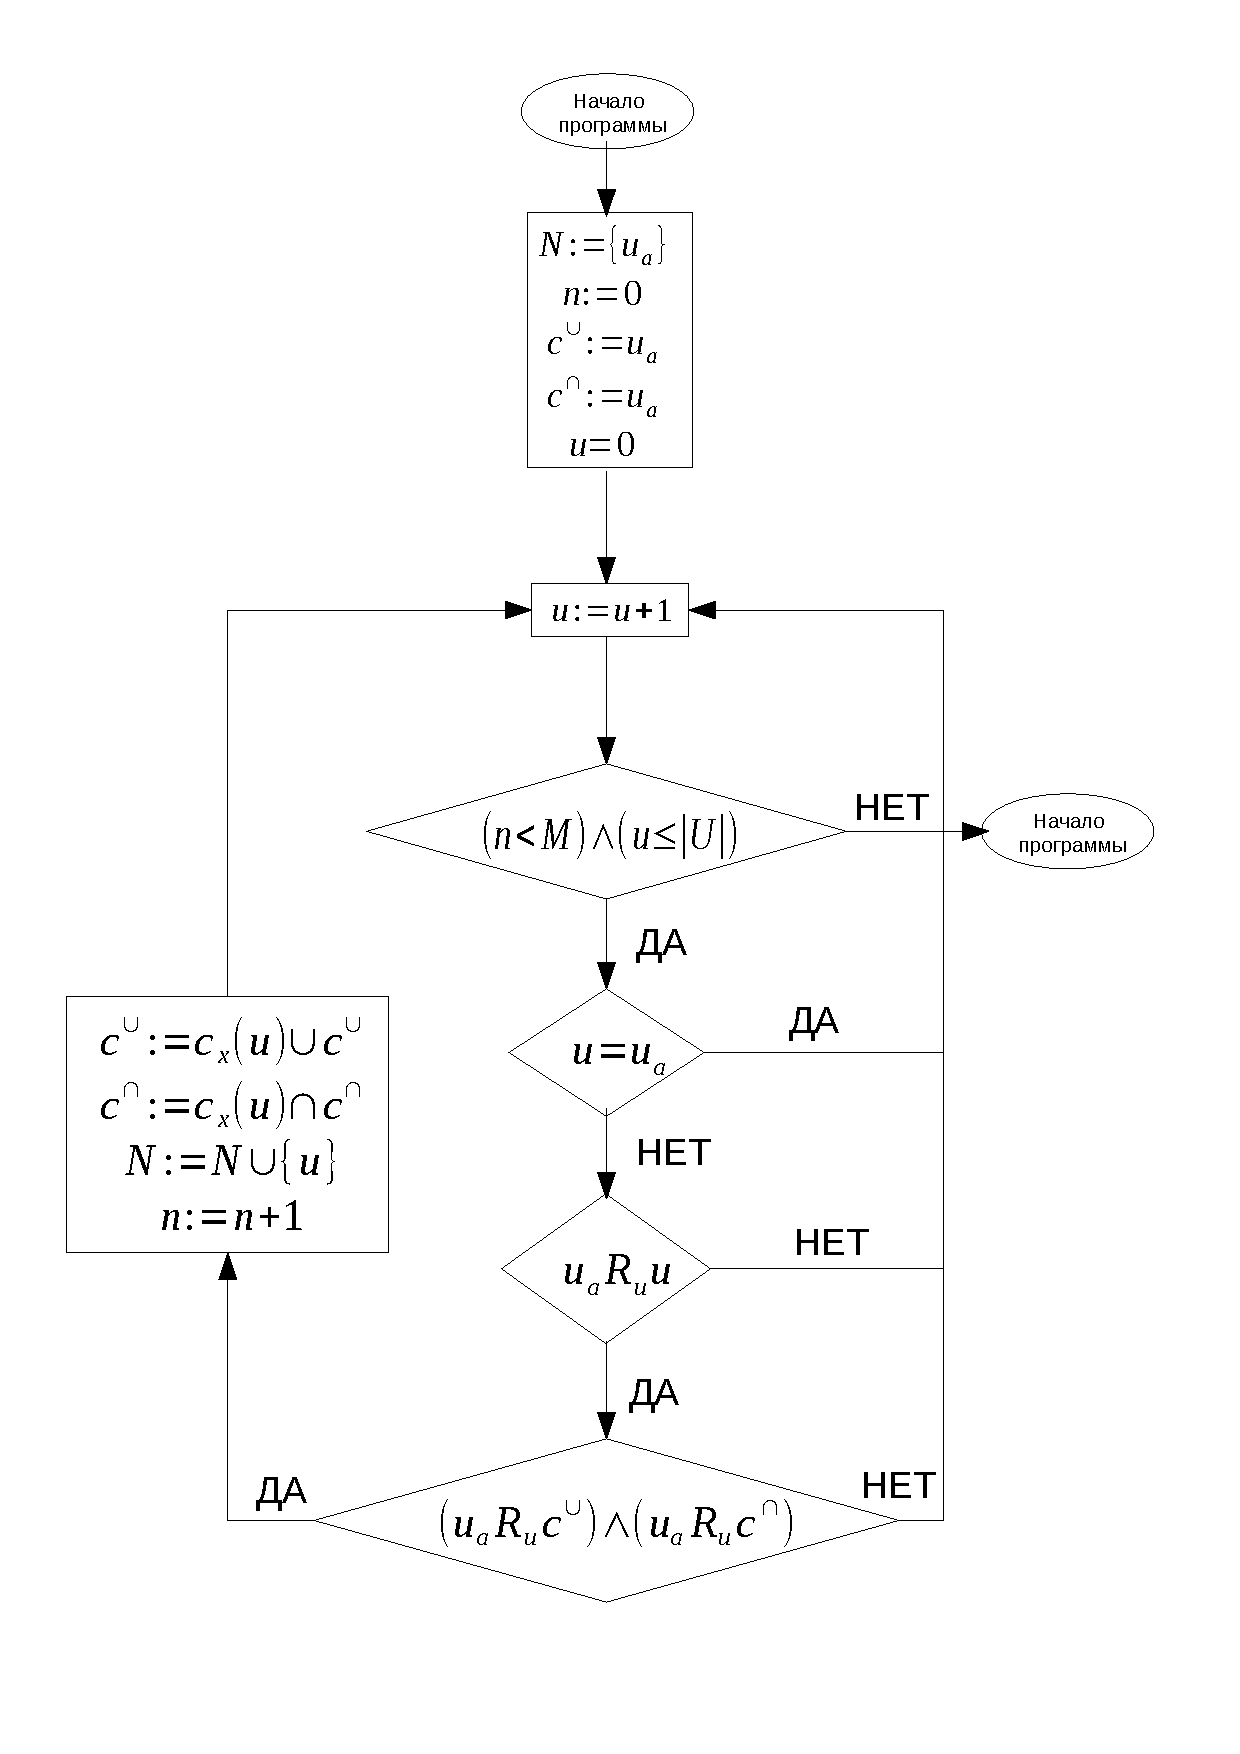
\includegraphics[width=5in,height=5in]{pics/alg-neighb.pdf}
%	\end{center}
%\end{figure}


%Для того, чтобы использовать контентную нечеткую модель для решения задач,
%необходимо задать правило $\Pi_f$, которое зависит от оценки сходства
%$\delta_c: X \times Y$. Если $X \neq I$, как для случая с коллаборативными
%системами, то решения не зависят от свойств и мощности исходных данных $P$.
%Нечеткая контентная модель является расширением коллаборативной по исходным
%данным, так как в качестве множества $X$ может быть использовано множество
%$I$, а $w_U(u, i) = \rho(u, i) \in P$.

%Проведем сравнение решений коллаборативной и нечеткой модели:
%\begin{enumerate}
%	\item качество решения: при применении $\Pi_C, \Pi_O$ в нечеткой модели
%		решение более эффективно. При применении $\Pi_f$ эффективность зависит
%		от дополнительного условия, как и в случае АКМ. Этим дополнительным
%		условием является аккуратность задания $\Pi_f$, что так же, как и в
%		случае с АКМ зависит от разработчиков. Однако для нечеткой модели
%		разработчик обладает большей свободой действий (в случае с АКМ
%		разработчик может менять только два параметра: функцию и ее пороговое
%		значение), поэтому вероятность получения эффективного решения выше.
%		Теоретически нечеткая модель более эффективна по критерию качества.
%		%Для нечеткой модели взаимосвязь между пользователем и объектом
%		%выносится в качестве динамического параметра модели в качестве
%		%$\Pi_f$, для АКМ такое взамисвязаывнаие является статическим и выражено
%		%эвристическим утверждением. Нечеткая модель может быть реализована один
%		%раз, изменения при ее использовании на разных исходных данных
%		%будут отражаться только на внешнем параметре $\Pi_f$.
%
%	\item стабильность: качество решений в нечеткой модели не
%		зависят от свойств исходных данных, так как правило вывода
%		зависит от задания $\delta_c: X \times Y$, где множество $P$
%		не фигурирует. Для коллаборативной модели $X = I$, а $w(u, i) = \rho(u,
%		)i$, поэтому АКМ зависит от свойств исходных данных. Нечеткая модель
%		более эффективна по критерию стабильности.
%		%Нечеткая модель
%		%может применяться и в тех случаях, когда $|P| = 0$, что невозможгно в
%		%случае с АКМ, поэтому для нечеткой модели не существует
%
%	\item вычислительная сложность: алгоритмы решений задач нечеткой контентной модели
%		обладают асимптотической сложность, меньшей на порядок асимптотических
%		сложностей алгоритмов решений АКМ, поэтому нечеткая модель более
%		эффективна по критерию вычислительной сложности.
%\end{enumerate}

{\bf Вывод}: разработана математическая модель РС, которая теоретически
более эффективна, чем АКМ, и является ее расширением.

%Вывод: при использовании и АКМ, и контентной нечеткой модели важен вклад
%разработчика и учет выдвигаемых требований для использо. Однако разработанная модель, в отличие от АКМ, гарантирует
%получение качественного решения, если разработчик учел выдвинутые требования
%аккуратного задания $\delta_c$.

%В первом случае от его выбора $\du, \di, \varepsilon_0$
%зависит выполнение достаточных свойств получения качественного решения.

%зависит качество получаемых решений. Однако, для АКМ существуют факторы,
%которые не зависят от разработчика, но при этом влияют на получаемое качество
%решения и на объективность оценки $\mathcal{E}_{topN}$.
%Для контентной нечеткой модели дополнительные факторы, влияющие на качество и
%на $\mathcal{E}$, отсутствуют.
%Поэтому эта модель гарантирует получение качественного решения,
%которое обладает меньшей асимптотической сложностью по сравнению с , и объективность показателя $\mathcal{E}$,
%если функция $\delta_c$ задана разработчиком аккуратно. Таким образом,

%\begin{table}[h]
%		  \begin{center}
%			\begin{tabular}{|c|c|c|}
%			  \hline
%				Параметры модели & Коллаборативная модель & Контентная модель   \\ \hline
%				Зависимость от $|P|$  & Да & Нет   \\ \hline
%				Зависимость от динамики  & & \\ и неоднородности $T^a_0,
%				T^a_{\bot}$  & Да & Нет   \\ \hline
%				%Зависимость от $X$ и $Y$  & Нет & Да   \\ \hline
%				Реализация $\rho: U \times I \rightarrow [0,1]$
%				& Косвенная, основана на эвристике & Формальная \\ \hline
%				Функция разработчика
%				& Обеспечить выполнение достаточных условий  & Определение
%				$\delta_c$\\ \hline
%			\end{tabular}
%		  \end{center}
%		\end{table}
